\documentclass[11pt, xcolor=dvipsnames,svgnames,x11names]{article}
\usepackage{xcolor}
\usepackage{xspace}
\usepackage{url}
\usepackage[colorlinks=true,bookmarks=false,linkcolor=black,urlcolor=blue,citecolor=black]{hyperref}
\usepackage{fancyhdr}
\usepackage[top=1in,bottom=1.2in,left=1in,right=1in]{geometry}
\usepackage{multicol}
\usepackage{pgfplots}
\usepackage{tikz}
\usetikzlibrary{circuits.logic.US, patterns}
\usepackage{mathpazo}
\usepackage{biolinum} 
\usepackage[all]{tcolorbox}
\usepackage{../Lectures/rahul_math}
\renewcommand{\familydefault}{\sfdefault}

% --- Custom Color Palette from Image ---
\definecolor{headerRed}{HTML}{A3403D} % Dark red from image top
\definecolor{patternBg}{HTML}{F2D9D7} % Light pinkish bg from image bottom
\definecolor{binaryText}{HTML}{D1A7A4} % Muted color for binary digits

% --- Background Pattern Setup ---
\usepackage[pages=all]{background}
\backgroundsetup{
scale=1,
color=black,
opacity=1,
angle=0,
contents={%
  \begin{tikzpicture}[remember picture,overlay]
    % Top Header Bar
    \fill[headerRed] (current page.north west) rectangle ([yshift=-1.2cm]current page.north east);
    % Bottom Binary Background
    \fill[patternBg] (current page.south west) rectangle ([yshift=3.5cm]current page.south east);
    % Decorative Line (from image)
    \draw[headerRed, line width=2pt] ([xshift=1in, yshift=-2.5cm]current page.north west) -- ([xshift=8in, yshift=-2.5cm]current page.north west);
    % Binary Text Overlay (Sample)
    \node[anchor=south, binaryText, font=\ttfamily\scriptsize, inner sep=0pt, yshift=1.5cm] at (current page.south) {
        \begin{tabular}{c@{\hspace{0.5em}}c@{\hspace{0.5em}}c@{\hspace{0.5em}}c@{\hspace{0.5em}}c@{\hspace{0.5em}}c@{\hspace{0.5em}}c}
        0 0 0 0 1 1 1 1 0 0 0 0 1 1 0 1 1 1 0 0 0 1 \\
        1 0 0 1 0 1 0 0 0 1 0 0 1 1 0 0 1 0 1 1 \\
        0 0 1 1 0 0 1 0 1 1 1 0 1 1 0 1 0 1 0 0 0 \\
        \end{tabular}
    };
  \end{tikzpicture}
}
}

% --- Header Styling ---
\makeatletter
\renewcommand{\maketitle}{%
    \vspace*{0.2cm}
    \begin{center}
        \begin{tcolorbox}[
            enhanced,
            colback=white,
            colframe=headerRed,
            arc=0mm,
            title={\textcolor{white}{\bfseries \@title}},
            coltitle=white,
            fonttitle=\bfseries\large,
            attach boxed title to top left={xshift=10pt, yshift=-\tcboxedtitleheight/2},
            boxed title style={sharp corners, colback=headerRed, frame hidden}
        ]
        \large
        \vspace{10pt}
        \noindent \textbf{Student Name:} \underline{\hspace{7cm}} \hfill \textbf{Points:} 30
        
        \vspace{10pt}
        \noindent \textbf{A Number:} \underline{\hspace{11cm}}
        \end{tcolorbox}
    \end{center}
    \vspace{10pt}
}
\makeatother

\newcommand{\hw}{Quiz 1}
\newcommand{\duedate}{Jan 22, 2026}

\pagestyle{fancy}
\fancyhf{}
\lhead{\small CPE 487/587, Spring 2026}
\rhead{\small \textit{\hw}}
\cfoot{\thepage}
\renewcommand{\headrulewidth}{0pt}

\def\checkmark{\tikz\fill[Green,scale=0.8](0,.35) -- (.25,0) -- (1,.7) -- (.25,.15) -- cycle;}

\begin{document}

\title{\hw}
\maketitle



\begin{enumerate}
\item Consider a Neural Network diagram:

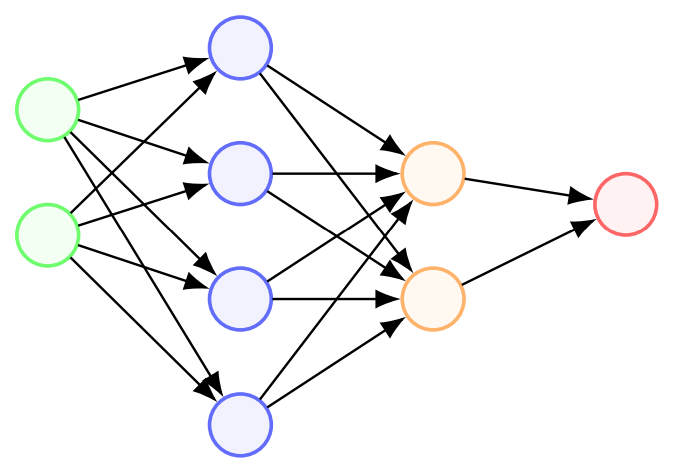
\includegraphics[width=0.5\linewidth]{figures/nn1.png}

If we are supplying two samples with two featurs (green bubbles), then what is the dimension of $W$s responsible for compressing 4 meta features to 2 meta features? For this assume that features in a feature matrix are along the column dimenions, and samples are along row dimensions.

\begin{enumerate}
\item $W_{4 \times 2}$ \checkmark
\item $W_{2 \times 4}$
\item $W_{4 \times 4}$
\item $W_{2 \times 2}$
\end{enumerate}



\item Consider an activation function as $\sigma(\xbf) = \frac{1}{1 + e^{-\xbf}}$ , if input is $\xbf = [1.09, 2.01, 3.0]$, the what is the dimension of $ A = \sigma(\xbf)$?

\begin{enumerate}

\item $3 \times 3$
\item $1$
\item Cannot be determined
\item $3$  \checkmark
\end{enumerate}

\item What does \texttt{curl} command do in a Linux machine?
\begin{enumerate}
\item It installs Python.
\item It searches websites for data.
\item It transfers data from server to client.  \checkmark
\item It creates a python virtual environment.
\end{enumerate}

\item Which Linux command is used for create a new directory?

\begin{enumerate}
\item cd
\item mkdir  \checkmark
\item ls
\item mv
\end{enumerate}

\item The function 
\begin{align*}
g(z) = \begin{cases}
1, \quad z \geq \theta\\
0, \quad otherwise
\end{cases}
\end{align*}
is fully differentiable.

\begin{enumerate}
\item True 
\item False  \checkmark
\end{enumerate}

\item Maximum value of the Sigmoid function $\sigma(\xbf) = \frac{1}{1 + e^{-x}}$ is

\begin{enumerate}
\item -1
\item +1  \checkmark
\item 0 
\item 0.5
\end{enumerate}

\item Consider a Neural Network definition:

          \begin{minted}[
                linenos,
                frame=lines,
                framesep=2mm,
                bgcolor=pink!10,
                fontsize=\footnotesize,
                breaklines
            ]{Python}
class QuizModel(nn.Module):
    def __init__(self):
        super().__init__()
        self.fc1 = nn.Linear(10, 5)
        self.relu = nn.ReLU()
        self.fc2 = nn.Linear(5, 2)

    def forward(self, x):
        x = self.fc1(x)
        x = self.relu(x)
        x = self.fc2(x)
        return x
\end{minted}

What is the size of the final output?

\begin{enumerate}
\item $2$  \checkmark
\item $5$
\item $1$
\item $2\times 5$
\end{enumerate}


\item Consider
\begin{align*}
\xbf = \begin{bmatrix}
1 \\ 2 \\ 4 \\ 6
\end{bmatrix}
\end{align*}
and 
\begin{align*}
\ybf = \fbf(\xbf) = \begin{bmatrix}
x_1 x_2 \\
x_1 + x_2\\
x_1x_2 + x_2x_3
\end{bmatrix}
\end{align*}

What is the size of Jacobian $J$?
\begin{enumerate}
\item  $4 \times 4$
\item $ 4\times 3$
\item $ 3\times 4$  \checkmark
\item $ 3 \times 3$
\end{enumerate}

\item Dropout 

\begin{enumerate}
\item randomly ignores a few neurons to create subnetwork on which training happens  \checkmark
\item randomly ignores a few samples to train on a subset of data samples
\item randomly ignores a few weights to train using remaining weights
\item randomly ignores a few layers to train using remaining layers
\end{enumerate}


\item A higher error on test set compared to training set denotes
\begin{enumerate}
\item A lack of generalizability of the trained model
\item Underfitting
\item Overfitting
\item Both (A) an (C)  \checkmark
\end{enumerate}

\end{enumerate}





\end{document}